\documentclass[12pt]{ctexart}
\usepackage[a4paper,margin=2.2cm]{geometry}
\usepackage{booktabs}
\usepackage{pgfplots}
\pgfplotsset{compat=1.18}

\title{Static Bending Comparison Report}
\author{Codex}
\date{2026-04-02 17:09:07}

\begin{document}
\maketitle

\section*{測試設定}
\begin{itemize}
\item 模型只包含 1D Timoshenko beam 與 2D Mindlin plate。
\item 數值腳本維持 test-style 主流程：\texttt{getElements -> prescribe! -> set𝝭!/set∇𝝭! -> 𝑎/𝑓 => elements}。
\item 固定常數：$E=10^8$，$\nu=0.3$，$\kappa=5/6$，$L=1.0$，$q=1.0$，$width/L=1.0$。
\item 掃描集合：$g \in \{1,2,3,5,10,15\}$，$h/L \in \{0.1,0.2,0.4\}$，mesh $\in \{10,20,40\}$，BC 目前只取 SS。
\end{itemize}

\section*{最佳結果總結}
\begin{table}[htbp]
\centering
\caption{1D Timoshenko Beam 最佳結果}
\begin{tabular}{ccccccccc}
\toprule
$h/L$ & BC & mesh & $g_b$ & $g_s$ & $g_{L2}$ & $L_2^w(\%)$ & $L_2^\phi(\%)$ & $w_h$ \\
\midrule
0.1 & SS & 40 & 2 & 1 & 5 & 0.153437 & 0.106088 & 1.59994e-06 \\
\bottomrule
\end{tabular}
\end{table}

\begin{table}[htbp]
\centering
\caption{2D Mindlin Plate 最佳結果}
\begin{tabular}{cccccccc}
\toprule
$h/L$ & BC & mesh & $g_{dom}$ & $g_{L2}$ & $L_2^w(\%)$ & $L_2^\phi(\%)$ & $w_h$ \\
\midrule
0.1 & SS & 16 & 2 & 5 & 161.821 & 264.796 & -9.74467e-07 \\
\bottomrule
\end{tabular}
\end{table}

\section*{代表性圖}
\begin{figure}[htbp]
\centering
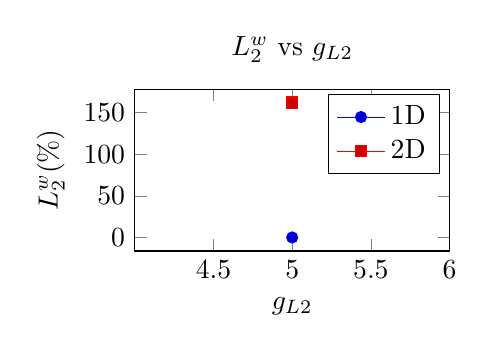
\begin{tikzpicture}
\begin{axis}[
    width=0.46\textwidth,
    height=0.30\textwidth,
    xlabel={$g_{L2}$},
    ylabel={$L_2^w(\%)$},
    title={$L_2^w$ vs $g_{L2}$},
    legend pos=north east,
]
\addplot+[mark=*] coordinates {(5,0.15343677166318123)};
\addlegendentry{1D}
\addplot+[mark=square*] coordinates {(5,161.82113437349918)};
\addlegendentry{2D}
\end{axis}
\end{tikzpicture}
\hfill
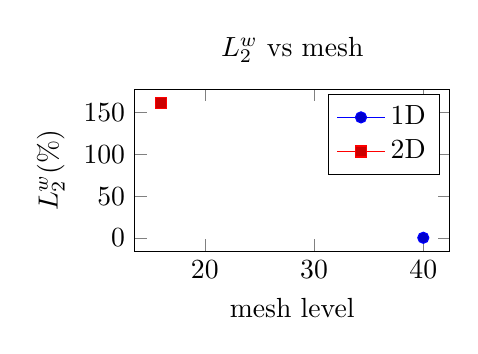
\begin{tikzpicture}
\begin{axis}[
    width=0.46\textwidth,
    height=0.30\textwidth,
    xlabel={mesh level},
    ylabel={$L_2^w(\%)$},
    title={$L_2^w$ vs mesh},
    legend pos=north east,
]
\addplot+[mark=*] coordinates {(40,0.15343677166318123)};
\addlegendentry{1D}
\addplot+[mark=square*] coordinates {(16,161.82113437349918)};
\addlegendentry{2D}
\end{axis}
\end{tikzpicture}
\caption{代表性曲線取樣固定為 $h/L=0.1$、BC=SS；1D 使用 $(g_b,g_s)=(2,1)$，2D 使用 $g_{dom}=2$。}
\end{figure}

\section*{簡短結論}
\begin{itemize}
\item 1D Timoshenko Beam 最佳 $L_2^w$ 出現在 $h/L=0.1$、mesh=40、$(g_b,g_s,g_{L2})=(2,1,5)$，$L_2^w=0.153437\%$。
\item 2D Mindlin Plate 最佳 $L_2^w$ 出現在 $h/L=0.1$、mesh=16、$g_{dom}=2$、$g_{L2}=5$，$L_2^w=161.821\%$。
\item 完整掃描資料已保存在 CSV，正文只保留代表性表格與圖形，以維持報告簡潔。
\end{itemize}

\end{document}
